\section{Prototyping}

\graphicspath{{./fig/}}	%specifying the folder for the figures

The coordinates calculated by the agents are \textit{virtual} ones ranging between 0.0 and 1.0. This prevents us from knowing the rendering-resolution and polluting code which has nothing to do with rendering with these implementation-details. Also this simulation could run without rendering-output or any rendering-frontend thus sticking to virtual coordinates is also very useful regarding this (but then again: what is the use of this simulation without any visual output=


\subsection{Reasoning}
Allowing to reason about a program is one of the most interesting and powerful features of a Haskell-program. Just by looking at the types one can show that there is no randomness in the simulation \textit{after} the random initialization, which is not slightest possible in the case of a Java, Scala, ReLogo or NetLogo solution. Things we can reason about just by looking at types:

\begin{itemize}
\item Concurrency involved?
\item Randomness involved?
\item IO with the system (e.g. user-input, read/write to file(s),...) involved?
\item Termination?
\end{itemize}

This all boils down to the question of whether there are \textit{side-effects} included in the simulation or not.

What about reasoning about the termination? Is this possible in Haskell? Is it possible by types alone? My hypothesis is that the types are an important hint but are not able to give a clear hint about termination and thus we we need a closer look at the implementation. In dependently-typed programming languages like Agda this should be then possible and the program is then also a 
proof that the program itself terminates.

reasoning about Heros \& Cowards: what can we deduce from the types? what can we deduce from the implementation?\\

Compare the pure-version (both Yampa and classic) with the IO-version of haskell: we loose basically all power to reason by just looking at the types as all kind of side-effects are possible when running in the IO-Monad.

in haskell pure version i can guarantee by reasoning and looking at the types that the update strategy will be simultaneous deterministic. i cant do that in java

TODO: implement haskell-version with shared-state (STM primitives) without using IO
TODO: implement haskell-version which defines abstract types for the simulation


\subsubsection{The type of a Simulation}
the type of a simulation: try to define the most general types of a simulation and then do reasoning about it

simulation :: Model -> Double -> Int -> [Model]

step :: Model -> Double -> Model

TODO: can we say something about the methods Model can/must/should support?

\subsection{Debugging \& Testing}
Because functions compose easier than classes \& objects (TODO: we need hard claims here, look for literature supporting this thesis or proof it by myself) it is also much easier to debug \textit{parts} of the implementation e.g. the rendering of the agents without any changes to the system as a whole - just the main-loop has do be adopted. Then it is very easy to calculate e.g. only one iteration and to freeze the result or to manually create agents instead of randomly create initial ones.

TODO: quickcheck \cite{claessen_quickcheck:_2000}


\subsection{Lazy Evaluation}
can specify to run the simulation for an unlimited number of steps but only the ones which are required so far are calculated.

\subsection{Performance}
Java outperforms Haskell implementation easily with 100.000 Agents - at first not surprising because of in-place updates of friend and enemies and no massive copy-overhead as in haskell. But look WHERE exactly we loose / where the hotspots are in both solutions. 1000.000 seems to be too much even for the Java-implementation.

\subsection{Numerical Stability}
The agents in the Java-implementation collapsed after a given number of iterations into a single point as during normalization of the direction-vector the length was calculated to be 0. This could be possible if agents come close enough to each other e.g. in the border-worldtype it was highly probable after some iterations when enough agents have assembled at the borders whereas in the Wrapping-WorldType it didn't occur in any run done so far. \\
In the case of a 0-length vector a division by 0  resulting in NaN which \textit{spread} through the network of neighbourhood as every agent calculated its new position it got \textit{infected} by the NaN of a neighbour at some point. The solution was to simply return a 0-vector instead of the normalized which resulted in no movement at all for the current iteration step of the agent. 


\subsection{Update-Strategies}
\begin{enumerate}
\item All states are copied/frozen which has the effect that all agents update their positions \textit{simultaneously}
\item Updating one agent after another utilizing aliasing (sharing of references) to allow agents updated \textit{after} agents before to see the agents updated before them. Here we have also two strategies: deterministic- and random-traversal.
\item Local observations: Akka
\end{enumerate}

\subsection{Different results with different Update-Strategies?}
Problem: the following properties have to be the same to reproduce the same results in different implementations: \\

Same initial data: Random-Number-Generators
Same numerical-computation: floating-point arithmetic
Same ordering of events: update-strategy, traversal, parallelism, concurrency

\begin{itemize}
\item Same Random-Number Generator (RNG) algorithm which must produce the same sequence given the same initial seed.
\item Same Floating-Point arithmetic
\item Same ordering of events: in Scala \& Actors this is impossible to achieve because actors run in parallel thus relying on os-specific non-deterministic scheduling. Note that although the scheduling algorithm is of course deterministic in all os (i guess) the time when a thread is scheduled depends on the current state of the system which can change all the time due to \textit{very} high number of variables outside of influence (some of the non-deterministic): user-input, network-input, .... which in effect make the system appear as non-deterministic due to highly complex dependencies and feedback.
\item Same dt sequence => dt MUST NOT come from GUI/rendering-loop because gui/rendering is, as all parallelism/concurency subject to performance variations depending on scheduling and load of OS.
\end{itemize}

It is possible to compare the influences of update-strategies in the Java implementation by running two exact simulations (agentcount, speed, dt, herodistribution, random-seed, world-type) in lock-step and comparing the positions of the agent-pairs with same ids after each iteration. If either the x or y coordinate is no equal then the positions are defined to be \textit{not} equal and thus we assume the simulations have then diverged from each other. \\
It is clear that we cannot compare two floating-point numbers by trivial == operator as floating-point numbers always suffer rounding errors thus introducing imprecision. What may seem to be a straight-forward solution would be to introduce some epsilon, measuring the absolute error: abs(x1 - x2) > epsilon, but this still has its pitfalls. The problem with this is that, when number being compared are very small as well then epsilon could be far too big thus returning to be true despite the small numbers are compared to each other quite different. Also if the numbers are very large the epsilon could end up being smaller than the smallest rounding error, so that this comparison will always return false. The solution would be to look at the \textit{relative error}: abs((a-b)/b) < epsilon. \\
The problem of introducing a relative error is that in our case although the relative error can be very small the comparison could be determined to be different but looking in fact exactly the same without being able to be distinguished with the eye. Thus we make use of the fact that our coordinates are virtual ones, always being in the range of [0..1] and are falling back to the measure of absolute error with an epsilon of 0.1. Why this big epsilon? Because this will then definitely show us that the simulation is \textit{different}. \\

The question is then which update-strategies lead to diverging results. The hypothesis is that when doing simultaneous updates it should make no difference when doing random-traversal or deterministic traversal => when comparing two simulations with simultaneous updates and all the same except first random- and the other deterministic traversal then they should never diverge. Why? Because in the simultaneous updates there is no ordering introduce, all states are frozen and thus the ordering of the updates should have no influence, \textit{both simulations should never diverge, \textbf{independent how dt and epsilon are selected}}. \\
Do the simulation-results support the hypothesis? Yes they support the hypothesis - even in the worst cast with very large dt compared to epsilon (e.g. dt = 1.0, epsilon = 1.0-12)

The 2nd hypothesis is then of course that when doing consecutive updates the simulations will \textit{always} diverge independent when having different traversal-strategies. \\
Simulations show that the selection of \textit{dt} is crucial in how fast the simulations diverge when using different traversal-strategies. The observation is that \textit{The larger dt the faster they diverge and the more substantial and earlier the divergence.}. Of course it is not possible to proof using simulations alone that they will always diverge when having different traversal-strategies. Maybe looking at the dynamics of the error (the maximum of the difference of the x and y pairs) would reveal some insight? \\

The 3rd hypothesis is that the number of agents should also lead to increased speed of divergence when having different traversal-strategies. This could be shown when going from 60 agents with a dt of 0.01 which never exceeded a global error of 0.02 to 6000 agents which after 3239 steps exceeded the absolute error of 0.1.

\subsection{Reproducing Results in different Implementations}
actors: time is always local and thus information as well. if we fall back to a global time like system time we would also fall back to real-time. anyway in distributed systems clock sync is a very non-trivial problem and inherently not possible (really?). thus using some global clock on a metalevel above/outside the simulation will only buy us more problems than it would solve us. real-time does not help either as it is never hard real time and thus also unpredictable: if one tells the actor to send itself a message after 100ms then one relies on the capability of the OS-timer and scheduler to schedule exactly after 100ms: something which is always possible thus 100ms are never hard 100ms but soft with variations.

qualitative comparison: print pucture with patterns. all implementations are able to reproduce these patterns independent from the update strategy

no need to compare individual runs and waste time in implementing RNGs, what is more interesting is whether the qualitative results are the same: does the system show the same emergent behaviour? Of course if we can show that the system will behave exactly the same then it will also exhibit the same emergent behaviour but that is not possible under some circumstances e.g. the simulation-runs of Akka are always unique and never comparable due to random event-ordering produced by concurrency \& scheduling. Also we don't have to proof the obvious: given the same algorithm, the same random-data, the same treatment of numbers and the same ordering of events, the outcome \textit{must} be the same, otherwise there are bugs in the program. Thus when comparing results given all the above mentioned properties are the same one in effect tests only if the programs contain no bugs - or the same bugs, if they \textit{are the same}. \\

Thus we can say: the systems behave qualitatively the same under different event-orderings.

Thus the essence of this boils down to the question: "Is the emergent behaviour of the system is stable under random/different/varying event-ordering?". In this case it seems to be so as proofed by the Akka implementation. In fact this is a very desirable property of a system showing emergent behaviour but we need to get much more precise here: what is an event? what is an emergent behaviour of a system? what is random-ordering of events? (Note: obviously we are speaking about repeated runs of a system where the initial conditions may be the same but due to implementation details like concurrency we get a different event-ordering in each simulation-run, thus the event-orderings vary between runs, they can be in fact be regarded as random).

\begin{figure}[H]
	\centering
  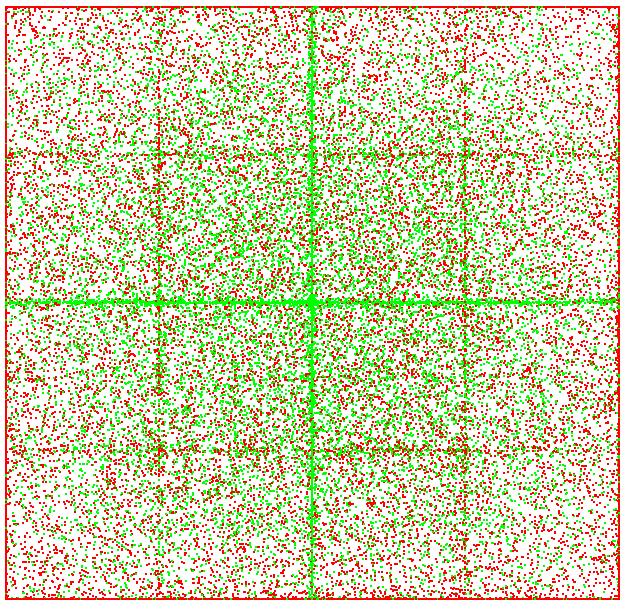
\includegraphics[width=1.0\textwidth, angle=0]{EMERGENT_PATTERN.png}
  	\caption{The emergent pattern used as criteria for qualitative comparison of implementations. Note the big green cross in the center and the smaller red crosses in each sub-sector. World-type is \textit{border} with 100.000 Agents where 25\% are Heroes.}
	\label{fig:EMERGENT_PATTERN}
\end{figure}


\subsection{Problem of RNG}
Have to behave EXACTLY The same: VERY difficult because of differing interfaces e.g. compare java to haskell RNGs.
Solution: create a deterministic RNG generating a number-stream starting from 1 and just counting up. The program should work also in this case, if not, something should be flawed!

Peer told me to implement a RNG-Trace: generate a list of 1000.0000 pre-calculated random-numbers in range of [0..1], store them in a file and read the trace in all implementations. Needs lots of implementation.

\subsection{Run-Time Complexity}
what if the number of agents grows? how does the run-time complexity of the simulation increases? Does it differ from implementation to implementation? The model is O(n) but is this true for the implementation?

\subsection{Simulation-Loops}
There are at least 2 parts to implementing a simulation: 1. implementing the logic of an agent and 2. implementing the iteration/recursion which drives the whole simulation

Classic \\
Yampa \\ TODO: use par to parallelize
Gloss \\
gloss provides means for simple simulation using simulate method. But: are all ABM systems like that?

\subsection{Agent-Representation}
Java: (immutable) Object
Haskell Classic: a struct
Haskell Yampa: a Signal-Function
Gloss: same as haskell classic
Akka: Actors

\subsection{EDSL}
simplify simulation into concise EDSL: distinguish between different kind if sims: continuous/discrete iteration on: fixed set, growing set, shrinking set, dynamic set. 